% Section drop-in: agentic adaptation of ErrorMap, results.
% Assumes the parent paper provides \documentclass, packages
% (booktabs, graphicx, tabularx), bibliography, etc.

\section{Behavioral Error Analysis on Agentic Trajectories}
\label{sec:agentic-errormap}

\subsection{Setup}

We adapt \textsc{ErrorMap}~\cite{ashury2026errormap} to long-horizon
agent trajectories produced by the Exgentic harness across the
design matrix of five agent harnesses (\texttt{claude\_code},
\texttt{tool\_calling}, \texttt{tool\_calling\_with\_shortlisting},
\texttt{smolagents\_code}, \texttt{openai\_solo}), five LM backbones
(Claude~Opus~4.5, DeepSeek-V3.2, Gemini~3~Pro~Preview, GPT-5.2,
Kimi-K2.5), and six benchmarks (\textsc{AppWorld},
\textsc{BrowseCompPlus}, \textsc{SWE-bench}, and three
$\tau^2$-bench variants). Of 13{,}652 sessions, we retained
4{,}551 failed sessions with full trajectory data; 76.7\% have a
peer-success ``gold'' trajectory from another agent or model on the
same task, used as the judge's reference solution.

The required adaptations are minimal: six binary-success entries
in \texttt{dataset2params}, a \mbox{$\sim$100-line} JSONL$\rightarrow$CSV
adapter that serializes \texttt{action}/\texttt{observation} pairs
and pairs each failure with a shared-\texttt{example\_id} gold row,
and a vocabulary refresh of five Jinja2 prompt templates
(\emph{model response} $\rightarrow$ \emph{agent's trajectory},
\emph{incorrect answer} $\rightarrow$ \emph{task failure},
\emph{model thinking} $\rightarrow$ root-cause guidance that admits
control-flow and tool-use errors). No schema or output-format
changes are made. We use \texttt{azure/gpt-5.5} as the judge,
\texttt{max\_workers=100}, the upstream default
\texttt{max\_num\_clusters=25}, and run end-to-end in 42~minutes for
\$246. We release the adapted code, the trajectory corpus
(142~MB compressed), and all analysis artifacts.

\subsection{Cleanup pass}

The first run produced 26 top-level categories with
\emph{Other}~$=$~25.8\%, far above the 4.8\% reported in
\textsc{ErrorMap}. Inspection of \emph{Other} revealed sensible
depth-2 sub-categories that were synonyms of existing top-levels
(e.g.\ ``Other/Premature Termination'' duplicating top-level
\emph{Premature Termination}). We applied a deterministic post-pass
that (i)~promotes depth-2 sub-categories of \emph{Other} via a
hand-curated synonym map, (ii)~merges two pairs of overlapping
top-levels (\emph{Search Recovery~+~Adaptation};
\emph{Escalation Timing~+~Protocol}), and (iii)~promotes five
depth-2 categories with no top-level counterpart to top-level
status. The result is a 27-category top-level taxonomy with
\emph{Other}~$=$~2.1\%---slightly below \textsc{ErrorMap}'s
coverage. The mapping is public and deterministic.

\subsection{Findings}

\paragraph{Prevalence is flat.}
The largest category (\emph{Premature Termination}) accounts for
only 8.1\% of failures and the top~10 cumulatively cover 57.5\%
(Table~\ref{tab:agentic-prevalence}). \textsc{ErrorAtlas}, by
contrast, has a strongly peaked top-five (53.7\% concentrated). Agent
failures, in our corpus, are more diverse.

\begin{table}[h]
\centering\small
\caption{Top-level agent failure categories with $\geq$1\%
prevalence (n$=$2{,}868 categorized records). \textbf{Bold} marks
categories with no direct counterpart in
\textsc{ErrorAtlas}-17~\cite{ashury2026errormap} or
\textsc{AgentErrorTaxonomy}-17~\cite{liu2025agentdebug}.}
\label{tab:agentic-prevalence}
\begin{tabular}{rlrr}
\toprule
\# & Category & n & \% \\
\midrule
1 & \textbf{Premature Termination}        & 232 & 8.1 \\
2 & Evidence Retrieval Omission           & 211 & 7.4 \\
3 & \textbf{Search Recovery \& Adaptation}& 183 & 6.4 \\
4 & Unsupported Fabrication               & 167 & 5.8 \\
5 & Tool Invocation Error                 & 167 & 5.8 \\
6 & Constraint Interpretation Error       & 157 & 5.5 \\
7 & \textbf{Escalation Handling}          & 151 & 5.3 \\
8 & Entity Resolution Error               & 143 & 5.0 \\
9 & Evidence Interpretation Error         & 119 & 4.1 \\
10 & \textbf{Diagnostic Protocol Error}    & 118 & 4.1 \\
11 & Action Execution Error                & 118 & 4.1 \\
12 & Candidate Verification Failure        & 115 & 4.0 \\
13 & \textbf{Validation Recovery Failure}  & 104 & 3.6 \\
14 & Quantitative Reasoning Error          & 97  & 3.4 \\
15 & \textbf{Remediation Omission}         & 81  & 2.8 \\
16 & Coverage Enumeration Omission         & 75  & 2.6 \\
17 & \textbf{Finalization Protocol Error}  & 73  & 2.5 \\
18 & \textbf{Unauthorized Action Execution}& 69  & 2.4 \\
19 & Policy Eligibility Error              & 67  & 2.3 \\
20 & \textbf{Query Formulation Error}      & 60  & 2.1 \\
21 & \textbf{Confirmation Handling Error}  & 43  & 1.5 \\
22 & \textbf{Authentication Handling Error}& 36  & 1.3 \\
\midrule
\multicolumn{2}{r}{Other (uncategorized)}  & 61  & 2.1 \\
\bottomrule
\end{tabular}
\end{table}

\paragraph{14 novel categories cover 42\% of failures.}
Mapping each of our 27 top-level categories to the closest fit in
\textsc{ErrorAtlas}-17 and \textsc{AgentErrorTaxonomy}-17, we find
6 covered, 7 partially overlapping, and 14 novel. Novel categories
cluster into two themes:
\emph{control-flow} (\emph{Premature Termination},
\emph{Search Recovery \& Adaptation},
\emph{Validation Recovery Failure}, \emph{Looping Behavior}),
which describe \emph{when} agents stop, retry, or persist; and
\emph{protocol adherence} (\emph{Escalation Handling},
\emph{Diagnostic Protocol Error}, \emph{Confirmation Handling Error},
\emph{Authentication Handling Error}, \emph{Unauthorized Action
Execution}), which describe violations of explicit task or
domain protocols. Both themes are visible only in multi-step
trajectories and have no QA analogue.

\paragraph{Per-model failure signatures.}
The five LM backbones produce visibly different failure mixes
despite comparable end-task accuracy (Figure~\ref{fig:agentic-per-model}).
DeepSeek-V3.2 and GPT-5.2 over-index on \emph{Premature Termination};
Kimi-K2.5 over-indexes on \emph{Unsupported Fabrication} and
\emph{Tool Invocation Error}; Claude~Opus~4.5 over-indexes on
\emph{Candidate Verification Failure} and \emph{Diagnostic Protocol
Error}; Gemini~3 Pro over-indexes on \emph{Search Adaptation
Failure} and \emph{Unsupported Fabrication}. These distinct
signatures echo the central \textsc{ErrorMap} thesis that aggregate
accuracy hides systematic differences in how models fail.

\begin{figure}[h]
\centering
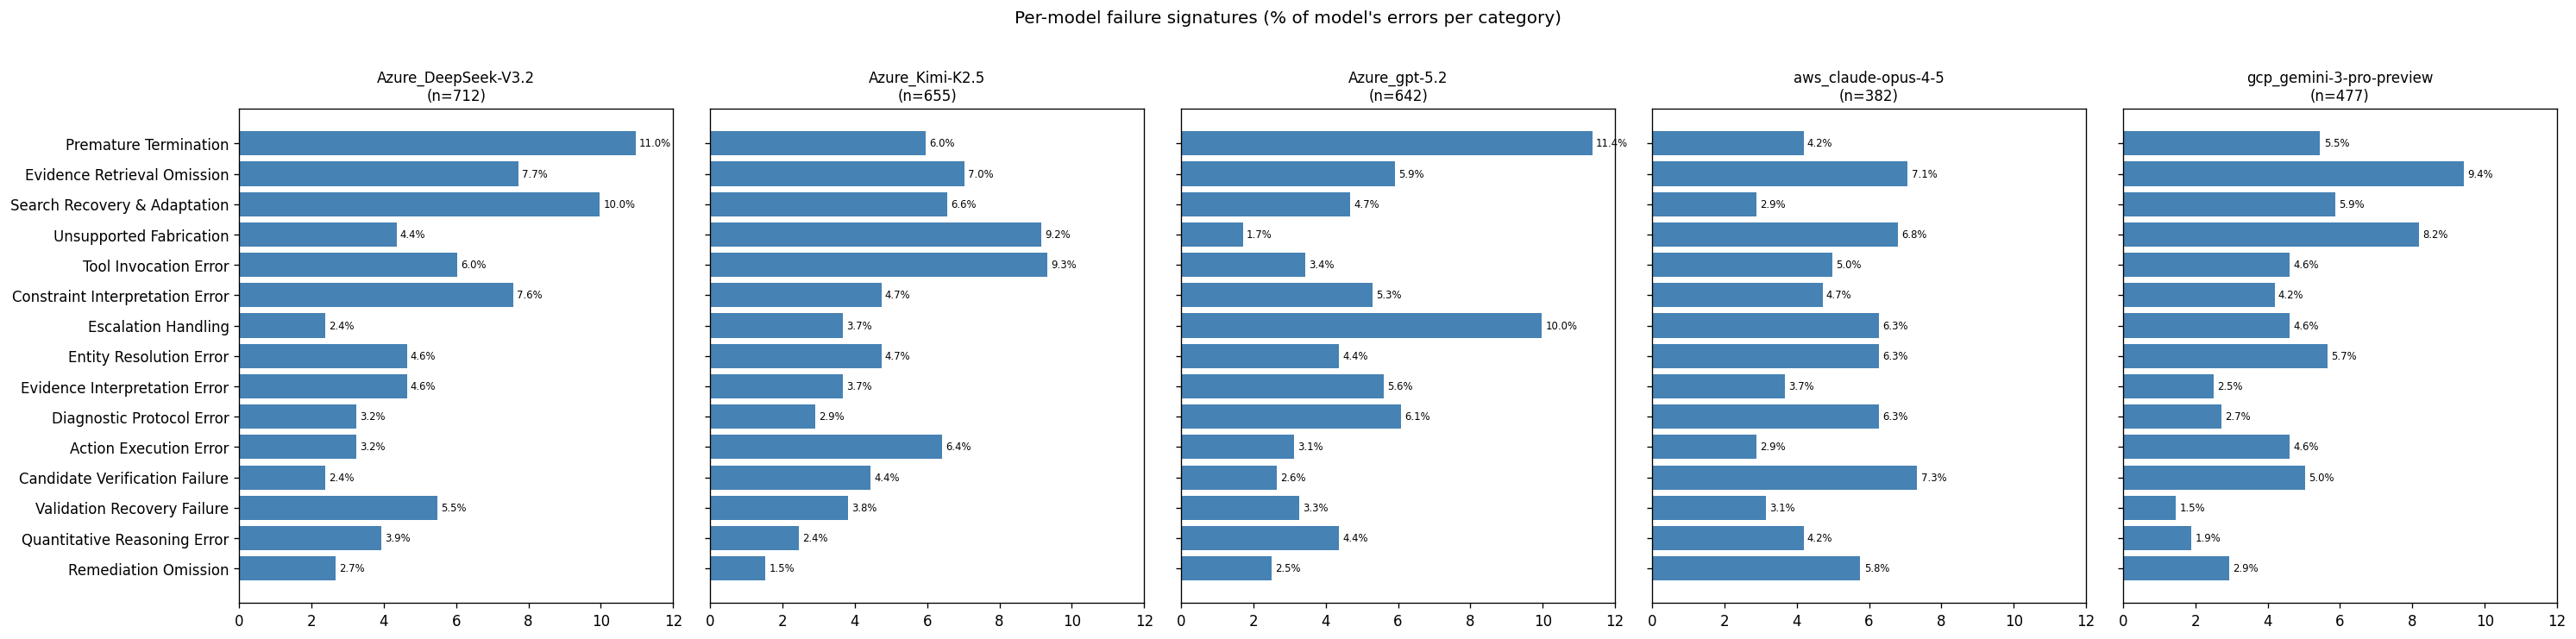
\includegraphics[width=\textwidth]{per_model_signatures.png}
\caption{Per-model failure signatures (top-15 categories,
column-normalized).}
\label{fig:agentic-per-model}
\end{figure}

\paragraph{Validation.}
Following \textsc{ErrorMap}'s protocol, we sample 100 labelled
records and present the judge with the assigned category vs.\ a
random alternative. The judge prefers the assigned label
\textbf{85\%} of the time (vs.\ 92\% in \textsc{ErrorMap}); the
gap is plausibly attributable to our larger 27-category vocabulary
and longer input contexts.
